% Fig. 6 - SCMA Factor Graph F4x6
% Compile: pdflatex fig6_factor_graph.tex
\documentclass[border=10pt]{standalone}
\usepackage{tikz}
\usepackage{amsmath}
\usetikzlibrary{arrows.meta, positioning, calc}

\begin{document}
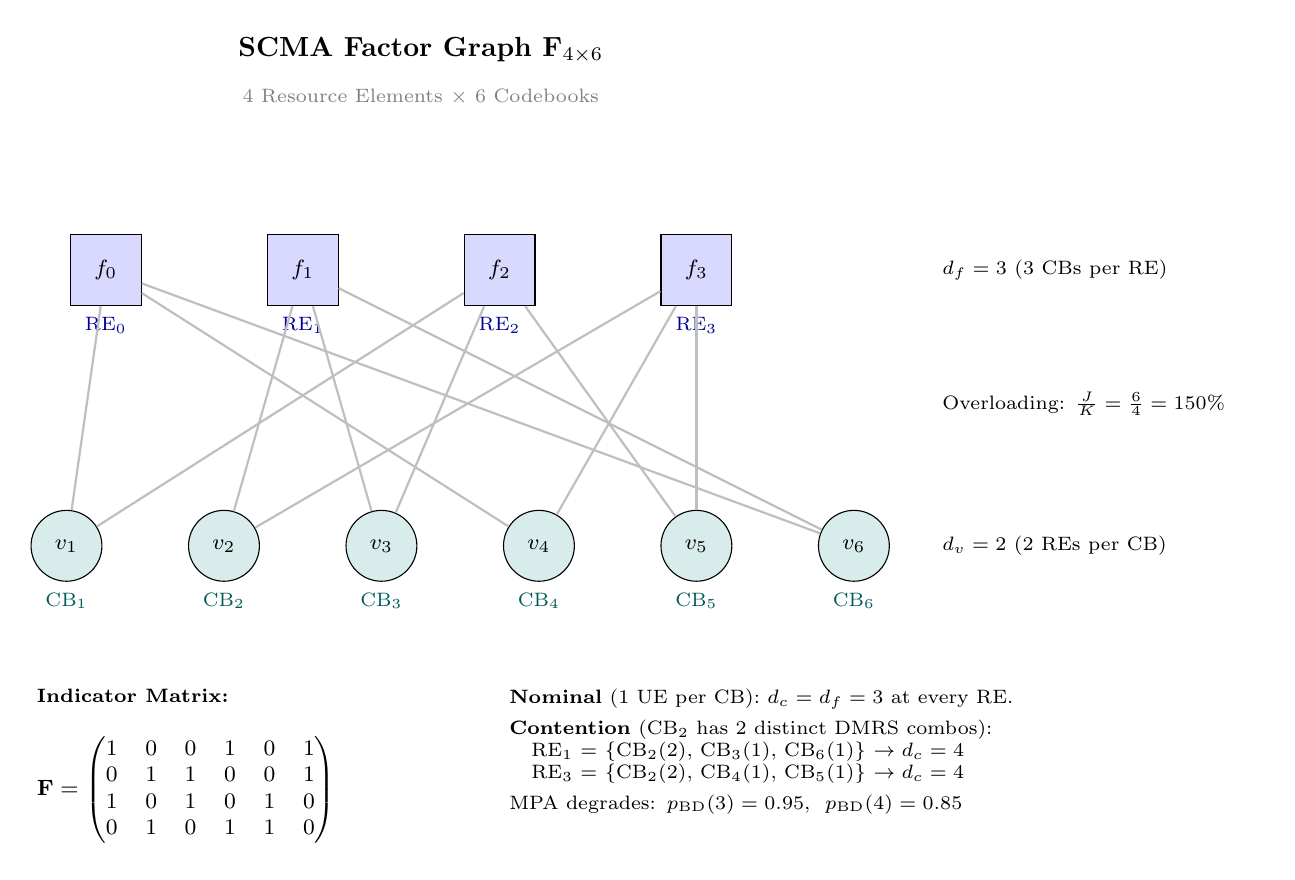
\begin{tikzpicture}[
    >=Stealth,
    font=\footnotesize,
    fn/.style={draw, rectangle, minimum width=0.9cm, minimum height=0.9cm,
               fill=blue!15, font=\footnotesize\bfseries},
    vn/.style={draw, circle, minimum size=0.9cm,
               fill=teal!15, font=\footnotesize\bfseries},
    edge/.style={thick, gray!50},
]

% === Title ===
\node[font=\normalsize\bfseries] at (4, 2.8)
     {SCMA Factor Graph $\mathbf{F}_{4 \times 6}$};
\node[font=\scriptsize, text=gray] at (4, 2.2)
     {4 Resource Elements $\times$ 6 Codebooks};

% === Function Nodes (top row) ===
\node[fn] (f0) at (0, 0) {$f_0$};
\node[fn] (f1) at (2.5, 0) {$f_1$};
\node[fn] (f2) at (5, 0) {$f_2$};
\node[fn] (f3) at (7.5, 0) {$f_3$};

\node[font=\scriptsize, text=blue!60!black] at (0, -0.7) {RE$_0$};
\node[font=\scriptsize, text=blue!60!black] at (2.5, -0.7) {RE$_1$};
\node[font=\scriptsize, text=blue!60!black] at (5, -0.7) {RE$_2$};
\node[font=\scriptsize, text=blue!60!black] at (7.5, -0.7) {RE$_3$};

% === Variable Nodes (bottom row) ===
\node[vn] (v1) at (-0.5, -3.5) {$v_1$};
\node[vn] (v2) at (1.5, -3.5) {$v_2$};
\node[vn] (v3) at (3.5, -3.5) {$v_3$};
\node[vn] (v4) at (5.5, -3.5) {$v_4$};
\node[vn] (v5) at (7.5, -3.5) {$v_5$};
\node[vn] (v6) at (9.5, -3.5) {$v_6$};

\node[font=\scriptsize, text=teal!70!black] at (-0.5, -4.2) {CB$_1$};
\node[font=\scriptsize, text=teal!70!black] at (1.5, -4.2) {CB$_2$};
\node[font=\scriptsize, text=teal!70!black] at (3.5, -4.2) {CB$_3$};
\node[font=\scriptsize, text=teal!70!black] at (5.5, -4.2) {CB$_4$};
\node[font=\scriptsize, text=teal!70!black] at (7.5, -4.2) {CB$_5$};
\node[font=\scriptsize, text=teal!70!black] at (9.5, -4.2) {CB$_6$};

% === Edges: F = [1 0 0 1 0 1; 0 1 1 0 0 1; 1 0 1 0 1 0; 0 1 0 1 1 0] ===
% f0 -> v1, v4, v6
\draw[edge] (f0) -- (v1);
\draw[edge] (f0) -- (v4);
\draw[edge] (f0) -- (v6);
% f1 -> v2, v3, v6
\draw[edge] (f1) -- (v2);
\draw[edge] (f1) -- (v3);
\draw[edge] (f1) -- (v6);
% f2 -> v1, v3, v5
\draw[edge] (f2) -- (v1);
\draw[edge] (f2) -- (v3);
\draw[edge] (f2) -- (v5);
% f3 -> v2, v4, v5
\draw[edge] (f3) -- (v2);
\draw[edge] (f3) -- (v4);
\draw[edge] (f3) -- (v5);

% === Right-side annotations ===
\node[font=\scriptsize, anchor=west] at (10.5, 0) {$d_f = 3$ (3 CBs per RE)};
\node[font=\scriptsize, anchor=west] at (10.5, -3.5) {$d_v = 2$ (2 REs per CB)};
\node[font=\scriptsize, anchor=west] at (10.5, -1.7)
     {Overloading: $\frac{J}{K} = \frac{6}{4} = 150\%$};

% === Indicator Matrix (properly formatted) ===
\node[font=\scriptsize, anchor=north west] at (-1, -5.2) {
    \textbf{Indicator Matrix:}
};
\node[anchor=north west] at (-1, -5.8) {
    $\mathbf{F} = \begin{pmatrix}
    1 & 0 & 0 & 1 & 0 & 1 \\
    0 & 1 & 1 & 0 & 0 & 1 \\
    1 & 0 & 1 & 0 & 1 & 0 \\
    0 & 1 & 0 & 1 & 1 & 0
    \end{pmatrix}$
};

% === dc explanation ===
\node[font=\scriptsize, anchor=north west, text width=9.5cm] at (5, -5.2) {
    \textbf{Nominal} (1 UE per CB): $d_c = d_f = 3$ at every RE.\\[3pt]
    \textbf{Contention} (CB$_2$ has 2 distinct DMRS combos):\\
    \quad RE$_1$ = \{CB$_2$(2), CB$_3$(1), CB$_6$(1)\} $\rightarrow d_c = 4$\\
    \quad RE$_3$ = \{CB$_2$(2), CB$_4$(1), CB$_5$(1)\} $\rightarrow d_c = 4$\\[3pt]
    MPA degrades: $p_{\text{BD}}(3) = 0.95$, \
    $p_{\text{BD}}(4) = 0.85$
};

\end{tikzpicture}
\end{document}
